\chapter{Opis projektnog zadatka}
		
		Potreba za kvalitetnom digitalizacijom bankarskih procesa i uvid u stanje pojedinih računa iz udobnosti doma od velikog su značaja kako za klijente, tako i za djelatnike banke. Cilj je ovog projekta razviti bankarski sustav: bazu podataka i sučelja prema bankarima, administratorima te krajnjim korisnicima banke, odnosno građanima.
		Korisnike dijelimo u nekoliko skupina : 
		\begin{packed_item}
			\item \textbf{administratori}, 
			\item \textbf{bankari},
			\item \textbf{službenici za odobravanje kreditnih zahtjeva građana} i 
			\item \textbf{korisnici u užem smislu} (građani).
		\end{packed_item}
		
		Svaka vrsta korisnika sustava ima svoj jedinstveni pogled u sustav putem web sučelja i Android aplikacije.
		
		\textit{\textbf{Neregistrirani korisnik}}, za registraciju u sustav upisuje svoj OIB i jedinstveni ključ koji je dobio od bankara. Nakon uspješnog unosa tih podataka, odabire korisničko ime i lozinku koji će mu u buduće služiti za prijavu u sustav. Ostale podatke o pojedinom korisniku kao što su: ime, prezime, adresa prebivališta, datum rođenja, e-mail adresa, sliku korisnika i dr., u sustav unosi bankarski službenik prilikom ugovaranja bilo kakve usluge banke.
		
		\textit{\textbf{Administrator}} u sustav ulazi unosom svoje korisničkog imea i lozinke koji mu daju pristup sustavu. On vidi popis svih korisnika sustava te može uređivati podatke za bilo koju vrstu korisnika, kao i dodavati te brisati same korisnike sustava. Jedina je osoba koja može kreirati račune ostalim djelatnicima banke.
		
		\textit{\textbf{Bankar}} svoj korisnički račun dobivaju od administratora. Ime, prezime, adresa prebivališta, OIB, datum rođenja, e-mail adresa i slika profila unaprijed su poznati podaci koje u sustav unosi administrator za svakog novog djelatnika. Pošto postanu dio kolektiva banke te nakon što administrator unese njihove podatke u sustav, u web aplikaciju unose korisničko ime i privremenu lozinku dobivenu od administratora sustava. Nakon prijave privremenom lozinkom, obavezni su odmah stvoriti novu lozinku. U sustavu imaju uvid u sve svoje osobne podatke, ali nemaju mogućnost izmjene tih podataka.
		Bankar nema uvid u popis korisnika sustava, niti u popis klijenata banke (građana). On može otvoriti, obrisati ili mijenjati profile klijenata. Kako bi pronašao profil nekog građana i uređivao ga ili brisao, dužan je unijeti OIB osobe za koju radi izmjenu u sustavu nakon čega mu se otvara profil te osobe (pretraga profila radi se po OIB-u građana). Također mu je dozvoljeno otvarati i zatvarati tekuće, žiro, štedne račune, ugovarati kredite, kreditne i debitne kartice za korisnike banke, aktivacija i deaktivacija kartica te obavljanje transakcija po računima klijenata.
		
		Svaki tekući račun ima dozvoljeno prekoračenje, a svaka kreditna kartica ima ugovoren limit.
		
		\textit{\textbf{Klijent}} dobiva dozvolu pristupa sustavu od bankara. Klijent banke ima uvid u sve podatke o svom profilu (ime, prezime, OIB, prebivalište, datum rođenja, slika profila i drugo), ali ih ne može mijenjati. Također, klijent može vidjeti sve svoje transakcijske račune, štedne račune, ugovorene kredite i kartice (debitne i kreditne). Klijent ne može mijenjati osobne podatke, podatke o računima, kreditima ili karticama. Klijent može vršiti prijenos sredstava između svojih transakcijskih računa (tekućeg, žiro ili štednog) ili na račune drugih klijenata banke. Također, klijent može ručno izvršiti uplatu kredit ili na kreditnu karticu kako bi umanjio iznos dugovanja ili otplatiti dugovanje ukupno.
		Klijent podnosi zahtjev za kreditom ili kreditnom karticom putem aplikacije ili u poslovnici banke gdje taj zahtjev unosi bankarski službenik. Za izradu kreditnog zahtjeva, u sustav se unosi iznos kredita, namjena kredita i rok otplate, dok kamatna stopa ovisi isključivo o namjeni kredita. Za izradu zahtjeva za kreditnom karticom, u sustav je potrebno unijeti samo vrstu kartice koja se traži (Mastercard, Visa, American Express, Diners, Discover i dr.).
		
		Svi korisnici moraju imati sliku profila (standardna slika za osobnu iskaznicu).
		
		Jednom mjesečno, u web aplikaciji, korisniku dolazi izvod po svim transakcijskim računima i kreditnim karticama u PDF i XLS obliku.
		
		\textit{\textbf{Službenici za odobravanje kreditnih zahtjeva građana}} imaju uvid u svoje osobne podatke koje ne mogu mijenjati. Također, vidljivi su im svi neobrađeni kreditni zahtjevi svih klijenata banke. Službenik može preuzeti bilo koji zahtjev na obradu te tada ima uvid u podatke o zahtjevu i sve podatke o klijentu koje banka posjeduje. Podaci o zahtjevu sadrže iznos zatraženog kredita, namjena kredita, kamatna stopa i vrijeme otplate ako se radi o zahtjevu za kredit, odnosno vrsta zatražene kreditne kartice ako se radi o zahtjevu za kreditnom karticom. Jedini podatak od navedenih koji se ne može mijenjati jest kamatna stopa jer ona ovisi o namjeni kredita. Službenik tada odobrava ili odbija zahtjev za kreditom, odnosno odobrava ili odbija kreditnu karticu kojoj ručno stvara određeni limit i kamatnu stopu.
		Nakon donesene odluke, korisnik tu odluku vidi u aplikaciji.
		
		Rate za kredite klijenata skidaju se automatski svaki mjesec na datum kojeg odredi administrator sustava i on je jedinstven za sve. U slučaju da na tekućem računu korisnika ne postoji dovoljno sredstava, ta se rata odgađa za jedan mjesec i bit će naplaćena zajedno s novom ratom idući mjesec.
		
		Dugovanje po kreditnoj kartici korisnik mora ručno otplatiti. Ako se u jednom mjesecu do unaprijed određenog datuma ne otplati račun u cijelosti, na preostali iznos zaračunava se kamata.
		
		Debitne kartice u sustavu prikazuju se odvojeno od tekućeg ili žiro računa kojem pripadaju. Može postojati račun bez debitne kartice, ali ne i debitna kartica bez računa. Odnosno, svaka debitna kartica mora biti vezana uz jedan račun.
		
		Važno je napomenuti da odvajamo pojam \textbf{profila korisnika sustava} od \textbf{korisničkog računa}.
		
		\textbf{Profil korisnika sustava} može postojati i bez korisničkog računa. On se sastoji od svih osobnih podataka korisnika (ime, prezime, OIB, adresa prebivališta, datum rođenja, e-mail adresa i slika profila), razine pristupa sustavu (administrator, bankar, službenik za odobravanje kredita ili klijent banke) te, ukoliko se radi o klijentu banke, svih njegovih ugovorenih usluga (transakcijskih računa, štednih računa, kredita, kreditnih kartica i debitnih kartica).
		
		Pod pojmom \textbf{korisničkog računa} podrazumijevamo način na koji korisnik pristupa podacima u sustavu i aktivnostima koji su mu dozvoljeni nad sustavom. Korisnički račun jest način kako korisnik sustava dobiva ovlast pregledavati sve podatke u sustavu koji su mu dozvoljeni. Njega definira korisničko ime i lozinka te svaki od vrste korisnika na drugačiji način (ranije definiran) dobiva korisnički račun. Svaki korisnički račun veže se uz jedan od korisničkih profila, odnosno korisnički račun ne može postojati bez profila korisnika.
		
		Primjeri ovakvog sustava mogu se pronaći u svim modernim, vodećim bankama u svijetu i u Hrvatskoj. Neki od njih prikazani su u nastavku.
		
		\begin{figure}[H]
			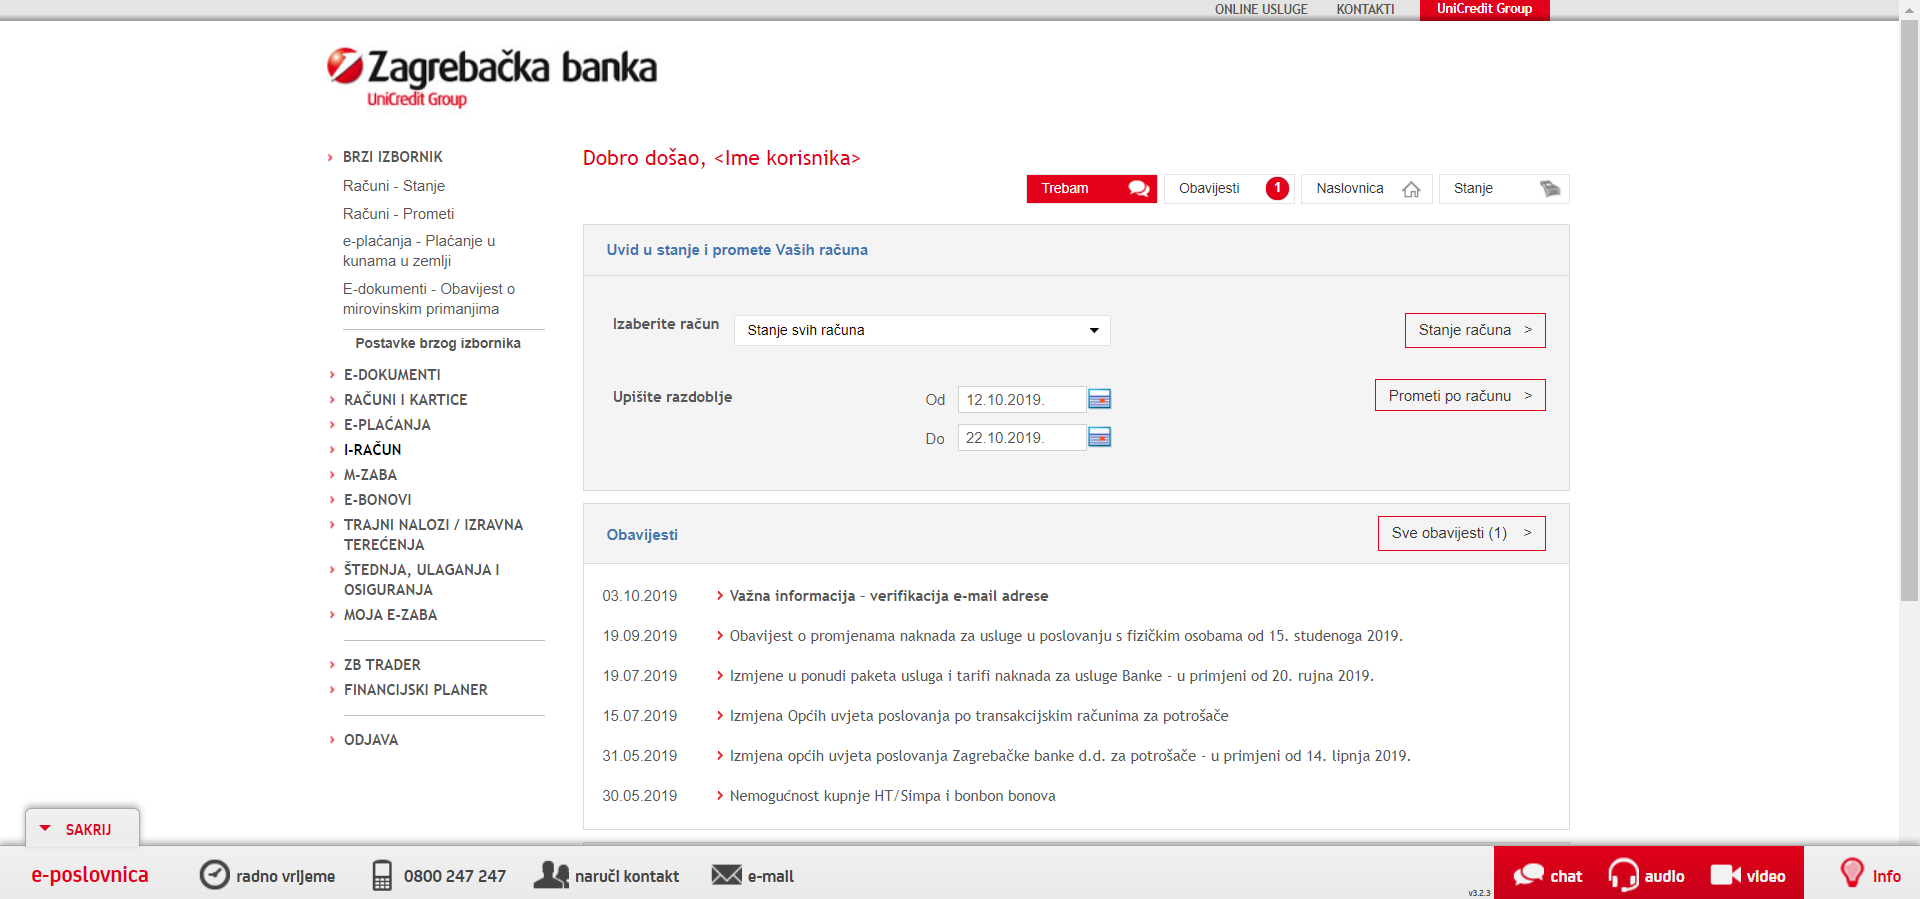
\includegraphics[scale=0.4]{slike/ezaba.PNG}
			\centering
			\caption{Usluga internet bankarstva Zagrebačke banke}
			\label{fig:ezaba}
		\end{figure}
	
		\begin{figure}[H]
			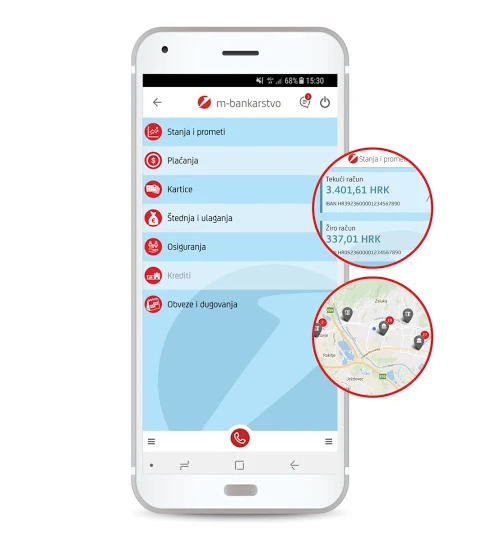
\includegraphics[scale=1]{slike/mzaba.PNG}
			\centering
			\caption{Usluga mobilnog bankarstva Zagrebačke banke}
			\label{fig:mzaba}
		\end{figure}
	
		\begin{figure}[H]
			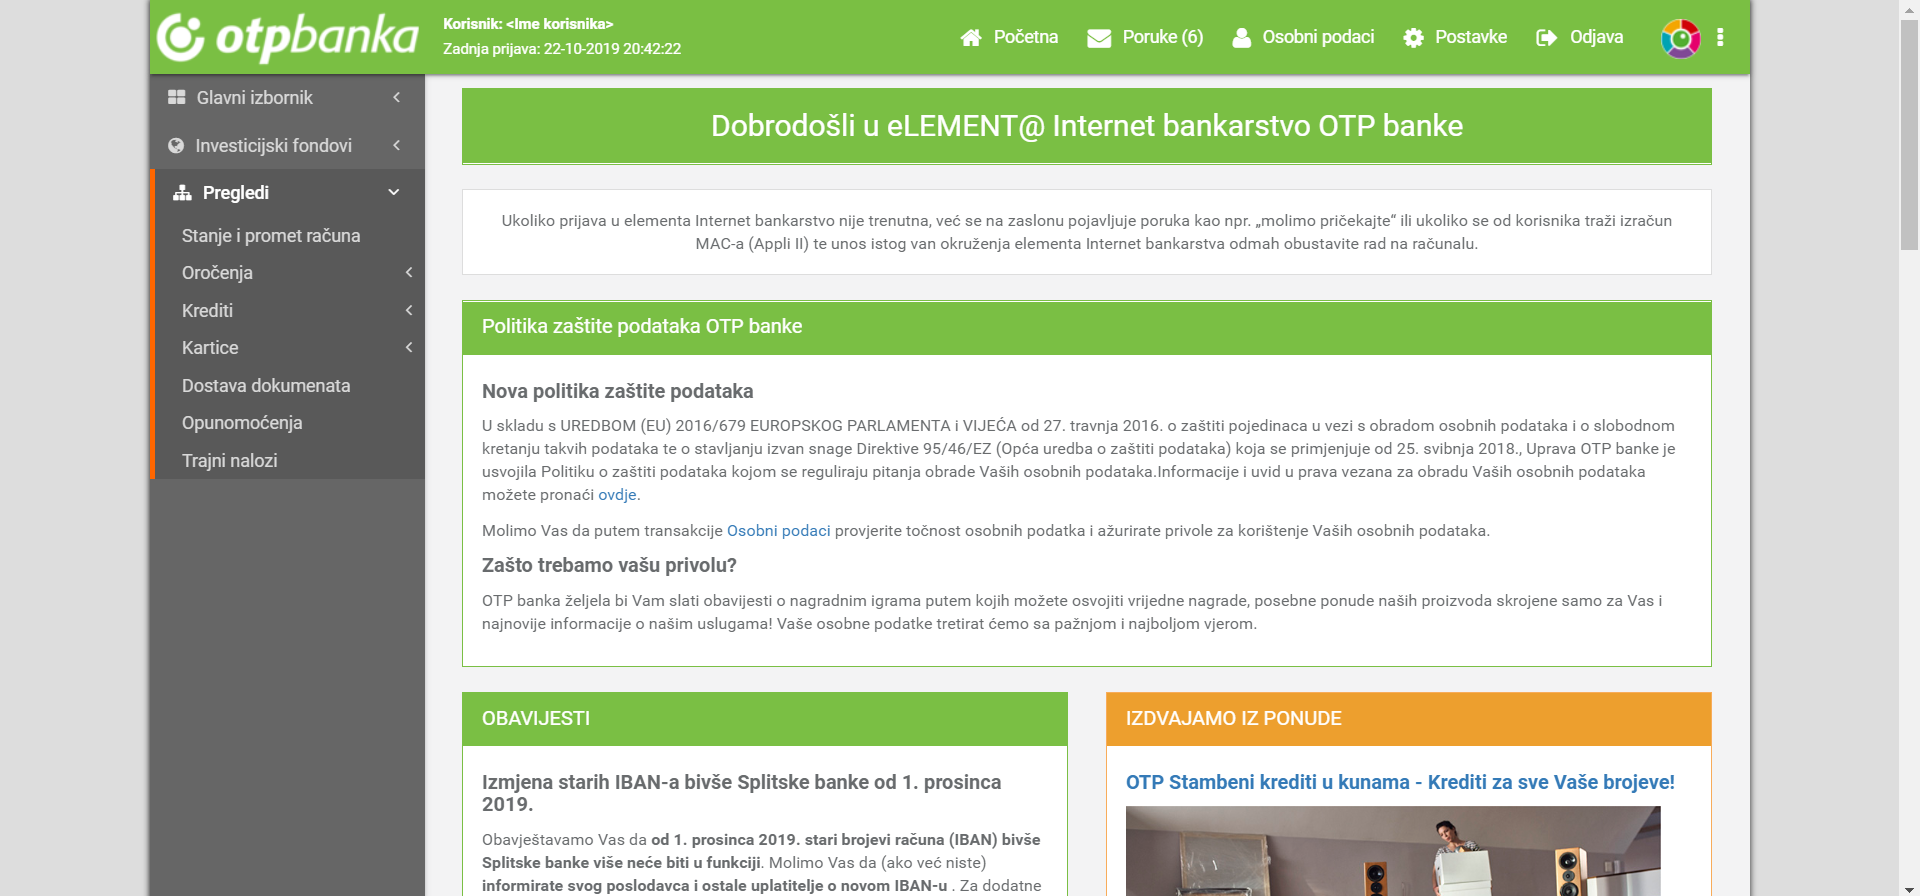
\includegraphics[scale=0.4]{slike/otp.PNG}
			\centering
			\caption{Usluga internet bankarstva OTP banke}
			\label{fig:otp}
		\end{figure}
	
		\begin{figure}[H]
			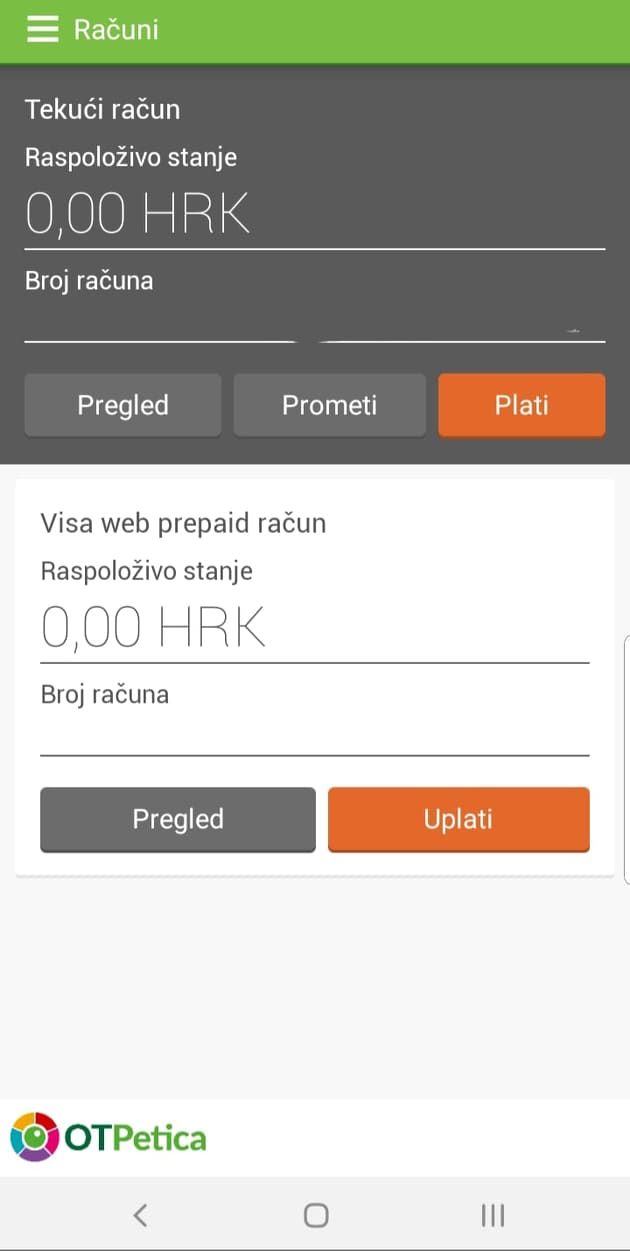
\includegraphics[scale=0.25]{slike/motp.JPG}
			\centering
			\caption{Usluga mobilnog bankarstva OTP banke}
			\label{fig:mzaba}
		\end{figure}
		
		\eject